\chapter{Fundamentals}\label{ch:fundamentals}
In this chapter should be explained how the used sensors work, which data they collect and how these data can be used for the purposes of mobile thermal mapping systems.
Furthermore the principals of localization and map creating with help of these sensors are discussed.

\section{Messurement Principles}\label{sec:messurementPrinciples}
Every sensor has different advantages and disadvantages which are caused by physical reasons or because improving would not allow to use them in a cost efficient mobile thermal mapping system.
But the disadvantages can be overcome by using the advantages of other sensors.
Each sensor type is presented on the basis of their fundamental functionality which shows their basic advantages and disadvantages.
The disadvantages can be larger depending on the implementation, manufacturing processes and use cases.

\subsection{LiDAR}\label{ssec:lidar}

\ac{LiDAR} sensors measures the range to a light reflecting object by sending out a pulse of directed light and measure the time until the reflection comes back.
Using a static laser beam allows only getting a range in one direction, but adding one or two movable mirrors allows to scan in two respective three dimensions. \todo{add source, image and formula for range calculation}

Something to the used light this needs to be in a specific spectrum not hurting the eyes and mostly not visible.
It should also be reflected by the most materials.
But in fact it's not getting reflected by glas.

\todo{need to be more precise}

This method bases on the reflection of the laser light but not all materials reflect all of the laser beam which leads to multiple echoes.
These echoes can be used to "look through" some materials like leaves. \todo{add source}

The range measurements are highly accurate but the more dimensions the more time is needed for one full measurement.
E.g. the Z+F PROFILER\circledR{} 9012\todo{add source} needs $20.41\si{ms}$ for a 2D scan but the Z+F IMAGER\circledR{} 5016 needs at least $22\si{s}$.

The output of a \ac{LiDAR} sensor depends on the number of dimensions they measure.
All of them measure a distance but for each additional dimension one angle is added.
But in case of 3D scanner the output format is often a 2.5D image.

\subsection{Thermal Camera}\label{ssec:thermalCamera}

\begin{wrapfigure}[12]{I}{0.55\textwidth}
	\centering
	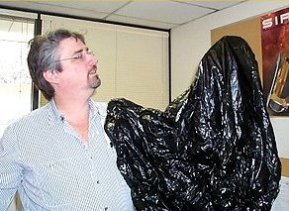
\includegraphics[height=2.8cm]{img/fundamentals/Human-Visible.jpg}
	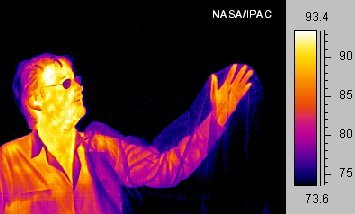
\includegraphics[height=2.8cm]{img/fundamentals/Human-Infrared.jpg}

	\caption{The RGB image in the left and the IR image on the right. The pictures show that IR radiation is blocked by the glasses but not by the thin plastic bag.}
	\label{fig:humanIRVIS}
\end{wrapfigure}

Every object emits \ac{EM} radiation which depends on the temperature of the object where the most of these emitted radiation is in the \ac{IR} spectrum.
Using the self emitted radiation has the advantages to be able to take measurements without any other active components like a lamp for classic RGB images.

\begin{wrapfigure}[27]{O}{0.45\textwidth}
	\centering
	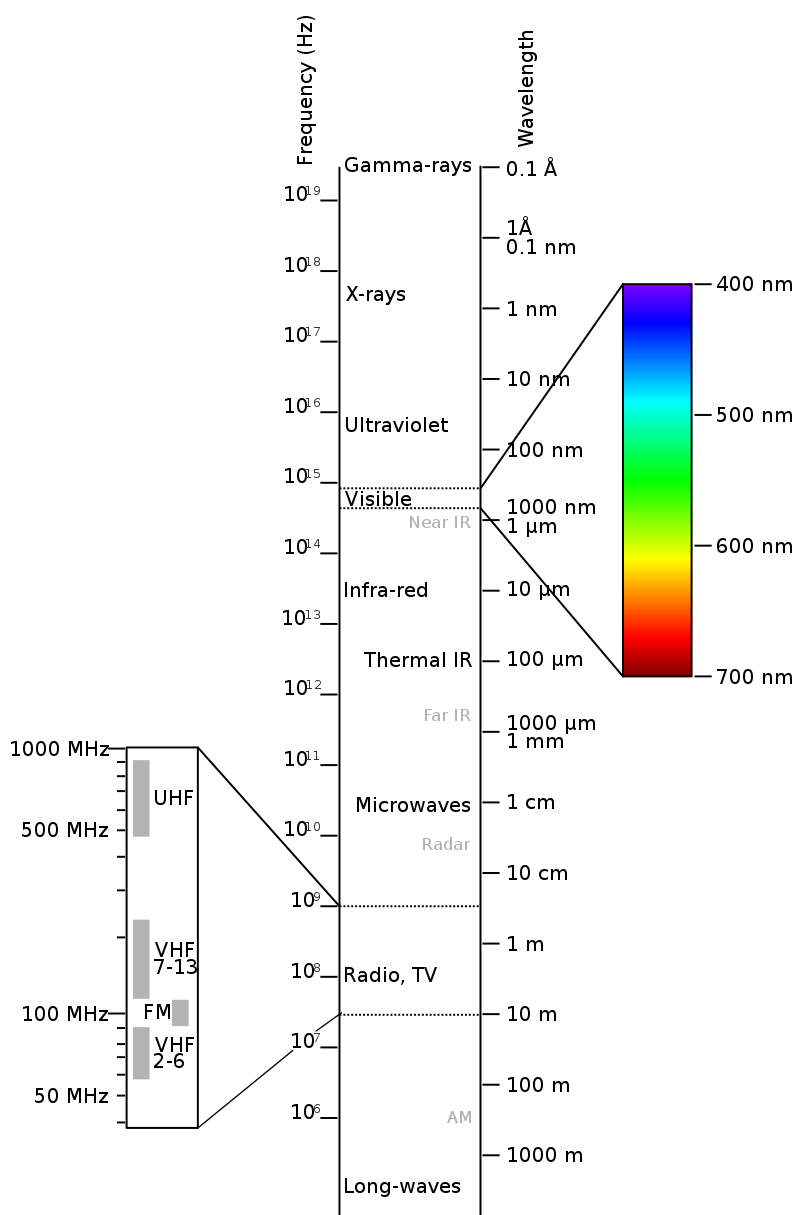
\includegraphics[width=0.45\textwidth]{img/fundamentals/em_spectrum.png}
	\caption{The electromagnetic spectrum with the visible light only covering a small part and the infrared as well as thermal infrared having a smaller frequency \cite{spectrum}
	}
	\label{fig:spectrum}
\end{wrapfigure}

Unlike RGB cameras thermal cameras doesn't use the \ac{VIS} but the \ac{IR} light.
Both lights can be described as \ac{EM} waves within an other spectrum.
\ac{VIS} covers only a tiny part with wave-lengths from $0.38$ to $0.78\si{\micro m}$, followed at longer wavelengths by the \ac{IR} from $0.78\si{\micro m}$ to $1\si{\milli m}$.
Within the \ac{IR} spectrum the \ac{TIR} is between $8\si{\micro m}$ and $14\si{\micro m}$\cite{Vollmer2017} (Figure \ref{fig:spectrum}).
But the same material can have different characteristics for these two spectrum.
As shown in figure \ref{fig:humanIRVIS} the glasses are blocking the \ac{IR} but the plastic bag not.

Like the common RGB cameras \ac{IR} cameras also use a lense to focus on the observed object and a sensor to transform the \ac{EM} waves in electric signals.
The lenses typically reflect parts of the \ac{IR} radiation which lowers the quality of the result.
To avoid these looses anti reflection coatings, band filters witch are known from the optical spectrum are used\cite{Vollmer2017} but also other materials are used for the lenses.
On the side of sensors there are two types which are used nowadays, the cooled and the uncooled sensors.
Comparing these two types the cooled is more precise but also higher in cost, size and weight.
An other drawback from the cooled sensors is that they need several minutes to cool down before they can take the first images.
Depending on the application the drawbacks can be accepted in favour of the higher precision.

Booth sensors don't measures the frequency, like the RGB sensors, but the intensity of \ac{TIR} radiation which leads to monochromatic images.
These images can be visualized in grey tone or pseudo colored images.

\subsection{Stereo Camera}\label{ssec:stereoCamera}
Stereo Cameras are typical two calibrated high definition RGB cameras observing the same scene.
For mobile mapping systems these two cameras are often arranged at the same horizontal plane with a distance of $10-12\si{cm}$.
This distance is named Baseline $B$.
Due to the distance between the two cameras each of them sees two slightly different pictures with different angles to the observed objects.
Because each cameras picture is distorted, each camera need a intrinsic calibration and to bring the cameras together they need a extrinsic calibration. \todo{better wording}

After the calibration the pictures can be rectified to proceed with matching single objects in the pictures.
The matching is necessary to calculate the disparity map which represents the depth of each pixel.
The matching between the objects can either be done manual or automatically while the manual matching is only possible in the post processing and the automatically can be used in real-time processing and post processing.
\todo{find/create image}
\todo{find primary source} 
\todo{maybe equation for }

\subsection{IMU}\label{ssec:imu}

A basic \ac{IMU} measures the linear acceleration using accelerometer and gyroscope to detect the rotational rate.
Typically these are measured over three perpendicular axis.
Modern \ac{IMU}s also use magnetometer to set the heading and barometer to estimate the hight.
Even more advanced \ac{IMU}s use \ac{GNSS} to improve their position with dead reckoning.

With the information about the acceleration and the rotation it is possible to calculate the current pose. \todo{formular}

Due the very fast accumulation of errors and the natural drift the pose is not reliable over a long term.
But in a short time frame an \ac{IMU} can provide very accurate data in a high frequency. \todo{source}

\section{Localization and Mapping}\label{sec:localizationAndMapping}

The main purpose of mobile mapping systems is to create a new map of an unknown environment with a portable platform.
These platforms can be attached to very small robots but also on bigger cars or even plains depending on their purpose.
A lot of mobile mapping systems use more than one sensor type to combine the advantages of each sensor to improve the result.

There are several ways to determine the current position.
\ac{GNSS} is a good option for outdoor environments but is not possible in locations where the signal from satellites can not be accessed by the receiver.

Mobile mapping describes the process of creating a map with a mobile platform using different sensors.
Determining the position can be done by \ac{GNSS} but that is not possible in areas where the
For these environments the \ac{SLAM} algorithm is a common approach.
\ac{SLAM} uses multiple sensors on a mobile mapping platform to determine the position and detect the surrounding environment at the same time.

\todo{map matching}
\todo{kalman filter}

